\documentclass[main.tex]{subfiles}
\ProvidesPackage{preamble}

\usepackage[nottoc]{tocbibind}
\usepackage[english]{babel}
\usepackage[utf8]{inputenc}
\usepackage[table]{xcolor}
\usepackage[nohead, nomarginpar, margin=1in, foot=.25in]{geometry}
\usepackage{tabularx}
\usepackage{graphicx}
\usepackage{float}
\usepackage[english]{babel}
\usepackage{paralist}
\usepackage{datetime}
\usepackage{afterpage}

\begin{document}

\subsection{Appendix A - User Manual}
As Thalia is a web application, it is accessible via the url: \url{TODO}. 

\begin{figure}[H]
   \centering
   
\includegraphics[scale=0.6]{08Appendices/081User/081Pictures/thalia_domain.png}
   \caption{Thalia Web (source: TODO)}
   \label{thalia_web}
\end{figure}

\subsubsection{Homepage}

By default the user should end up on the homepage, although some other pages are accessible as well given the correct url. 

\begin{figure}[H]
   \centering
   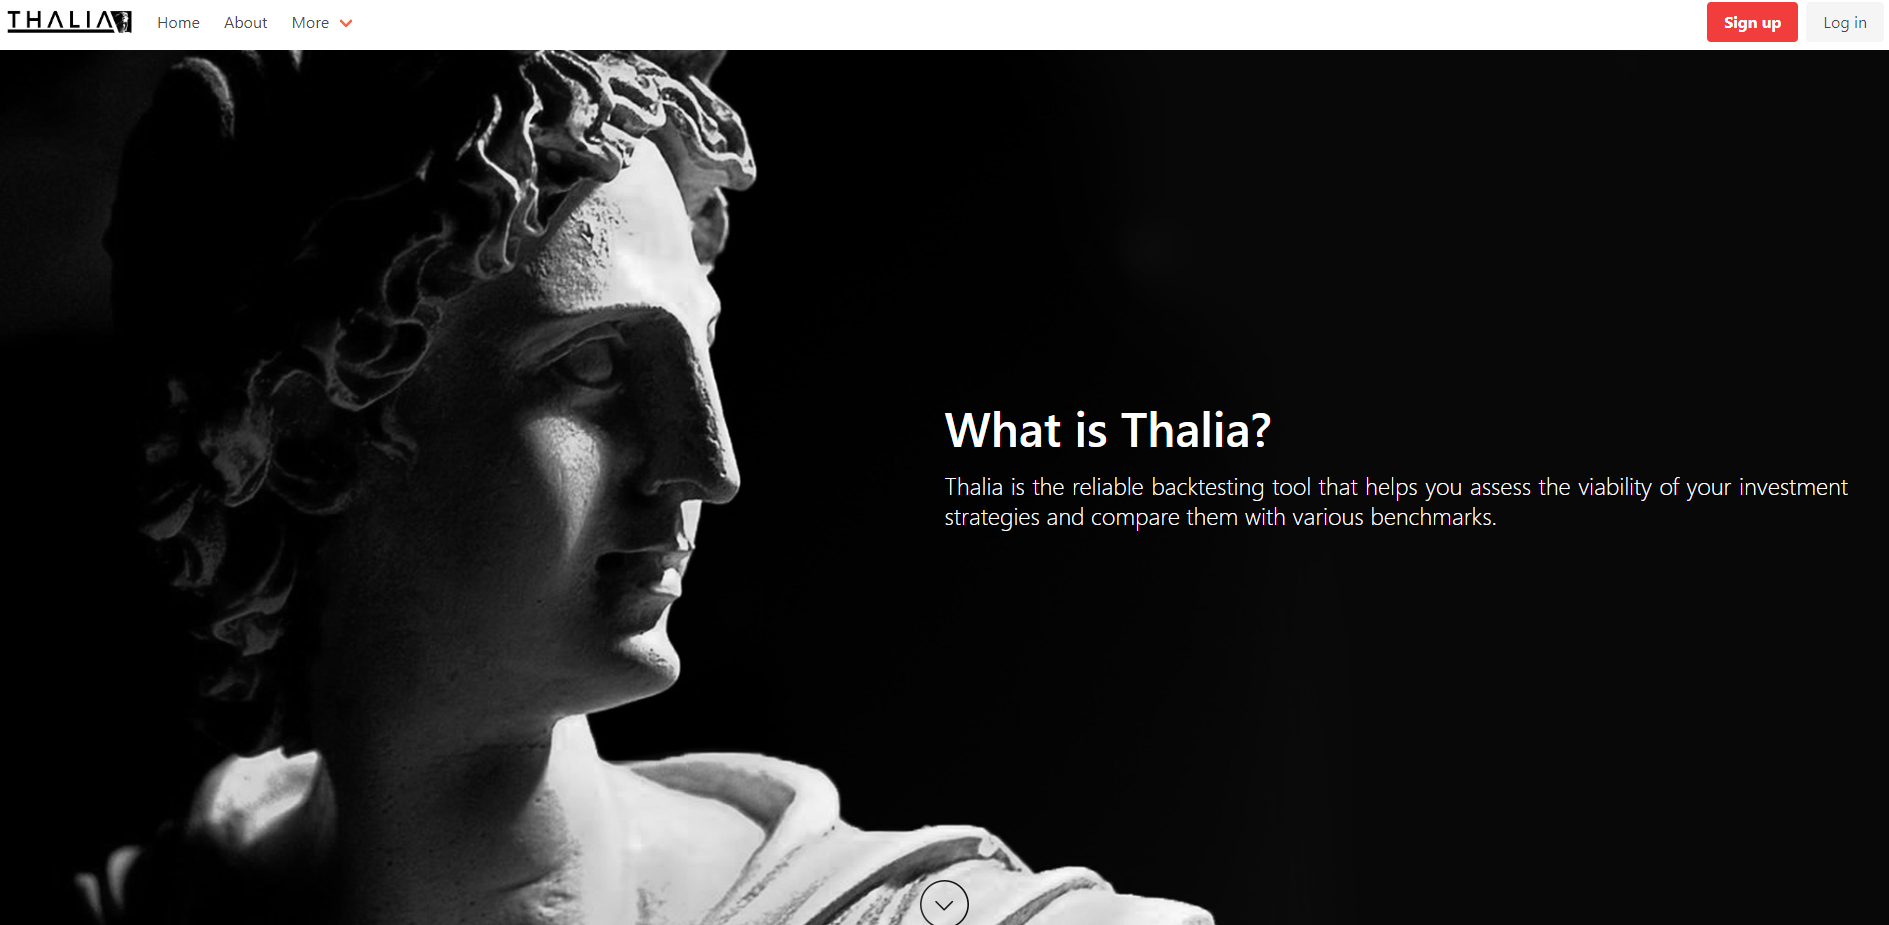
\includegraphics[width=\textwidth]{08Appendices/081User/081Pictures/homepage.png}
   \caption{Thalia Homepage (source: TODO)}
   \label{thalia_home}
\end{figure}

The purpose of the homepage is to provide a cover to our application. As the users scrolls down he or she can read some fundamental information on Thalia and the backtesting process.
As mentioned previously in our section of feasibility analysis \ref{TODO}, we do not wish users to blindly jump into the process of backtesting, this we felt the necessity to provide
some basic information on the process. A link at the end of the description then leads to the about page.

Scrolling further down the user may encounter a small register form, or in case the user is logged in, a link to the dashboard, ie. the main application.

\begin{figure}[H]
   \centering
   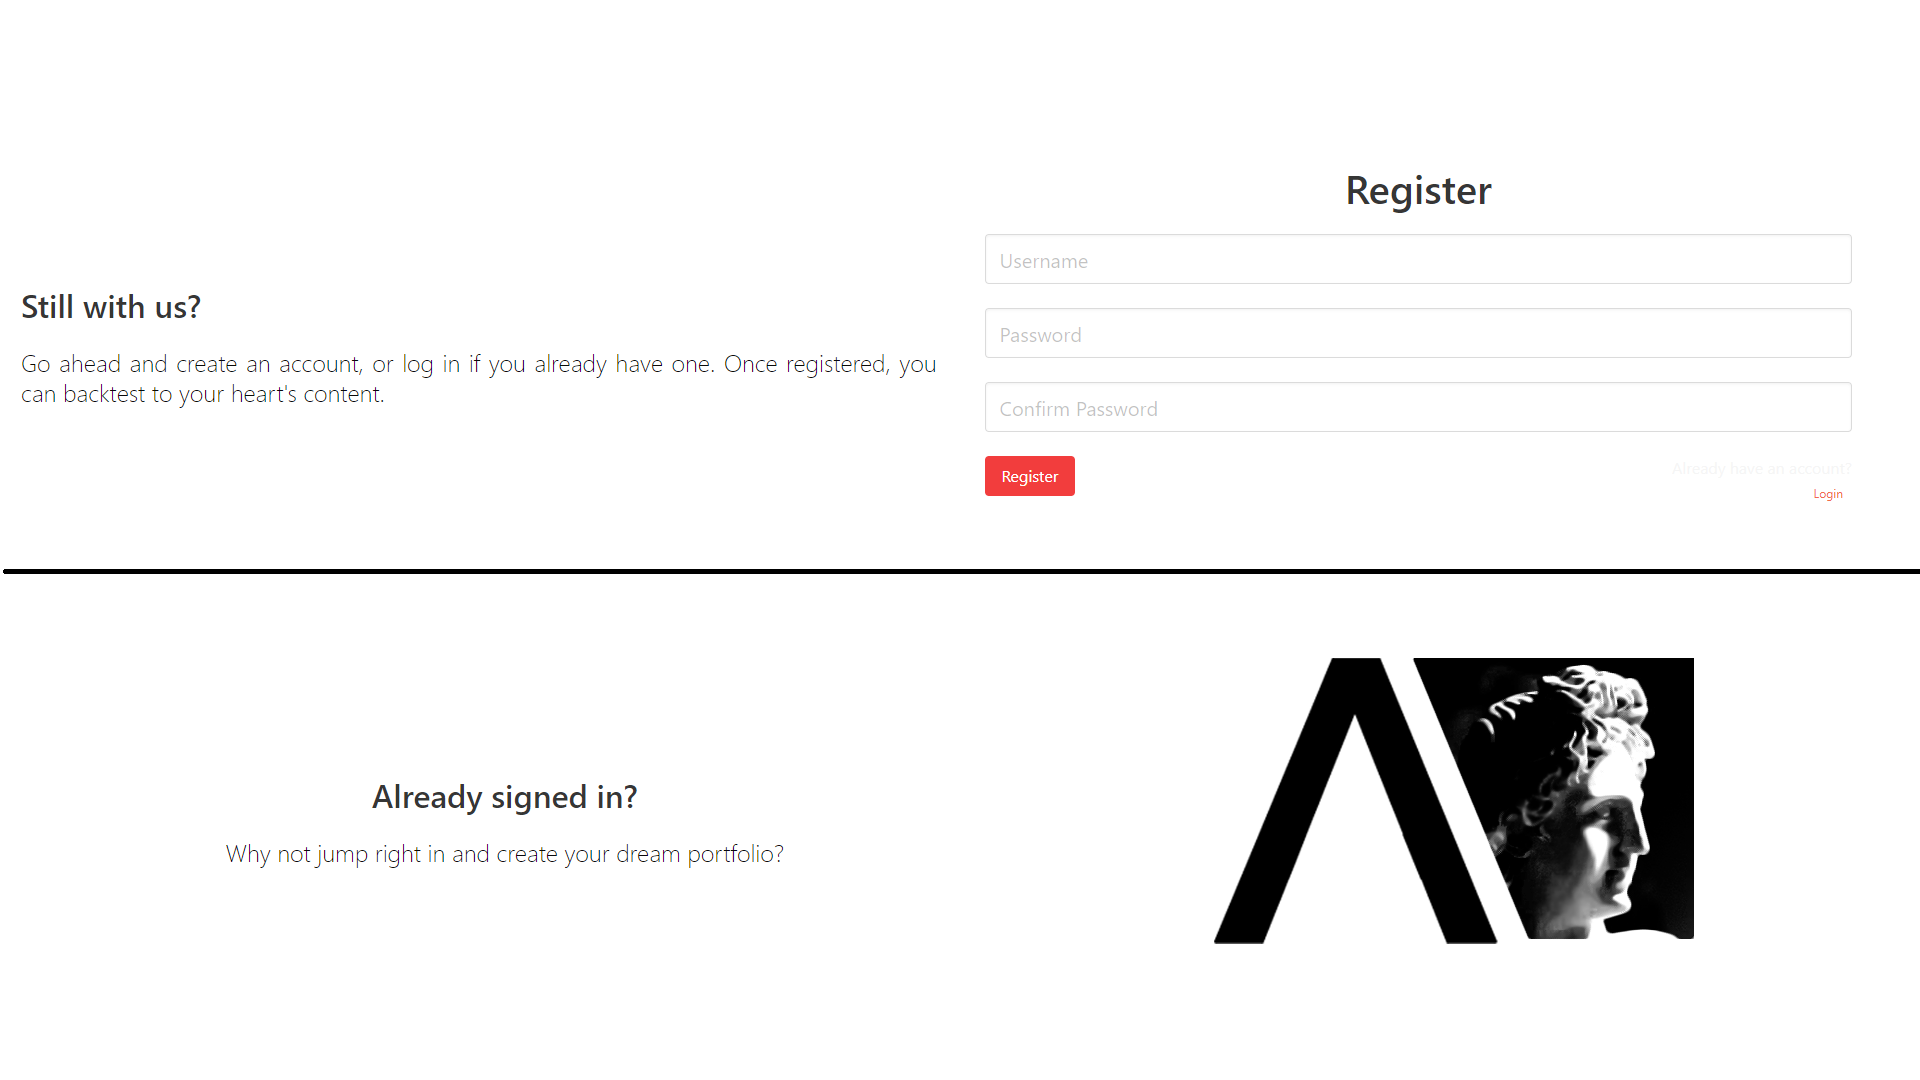
\includegraphics[width=\textwidth]{08Appendices/081User/081Pictures/homepage_bottom.png}
   \caption{Thalia Homepage Side by side (source: TODO)}
   \label{thalia_home_bottom}
\end{figure}

\subsubsection{About Page}

The About Page of our application is to provide a more detailed introduction to the problem domain, and is available at \url{TODO}.
The user can arrive at this page either by directly typing in the url, clicking on the learn more option on the Homepage, or by navigating here using the navbar option.

\begin{figure}[H]
   \centering
   
\includegraphics[width=\textwidth]{08Appendices/081User/081Pictures/navbar.png}
   \caption{Thalia Navbar (source: TODO)}
   \label{thalia_navbar}
\end{figure}

Our About Page looks as follows:

\begin{figure}[H]
   \centering
   \includegraphics[width=\textwidth]{08Appendices/081User/081Pictures/about_page.png}
   \caption{Thalia About Page (source: TODO)}
   \label{thalia_about}
\end{figure}

\subsubsection{Log In and Sign Up Pages}

TODO if we introduce extra  fields or regex for pw.

In case the User is not yet logged in, links for the Log In and Sign Up pages are visible on the navbar. In addition they are directly available at \url{TODO} and \url{TODO}.
Both of these forms are quite common, with the login requiring:

\begin{itemize}
    \item Username
    \item Password
    \item (Optional) Remember me
\end{itemize}

For signing up, the fields are:

\begin{itemize}
    \item Username
    \item Password
    \item Confirm Password
\end{itemize}

\begin{figure}[H]
   \centering
   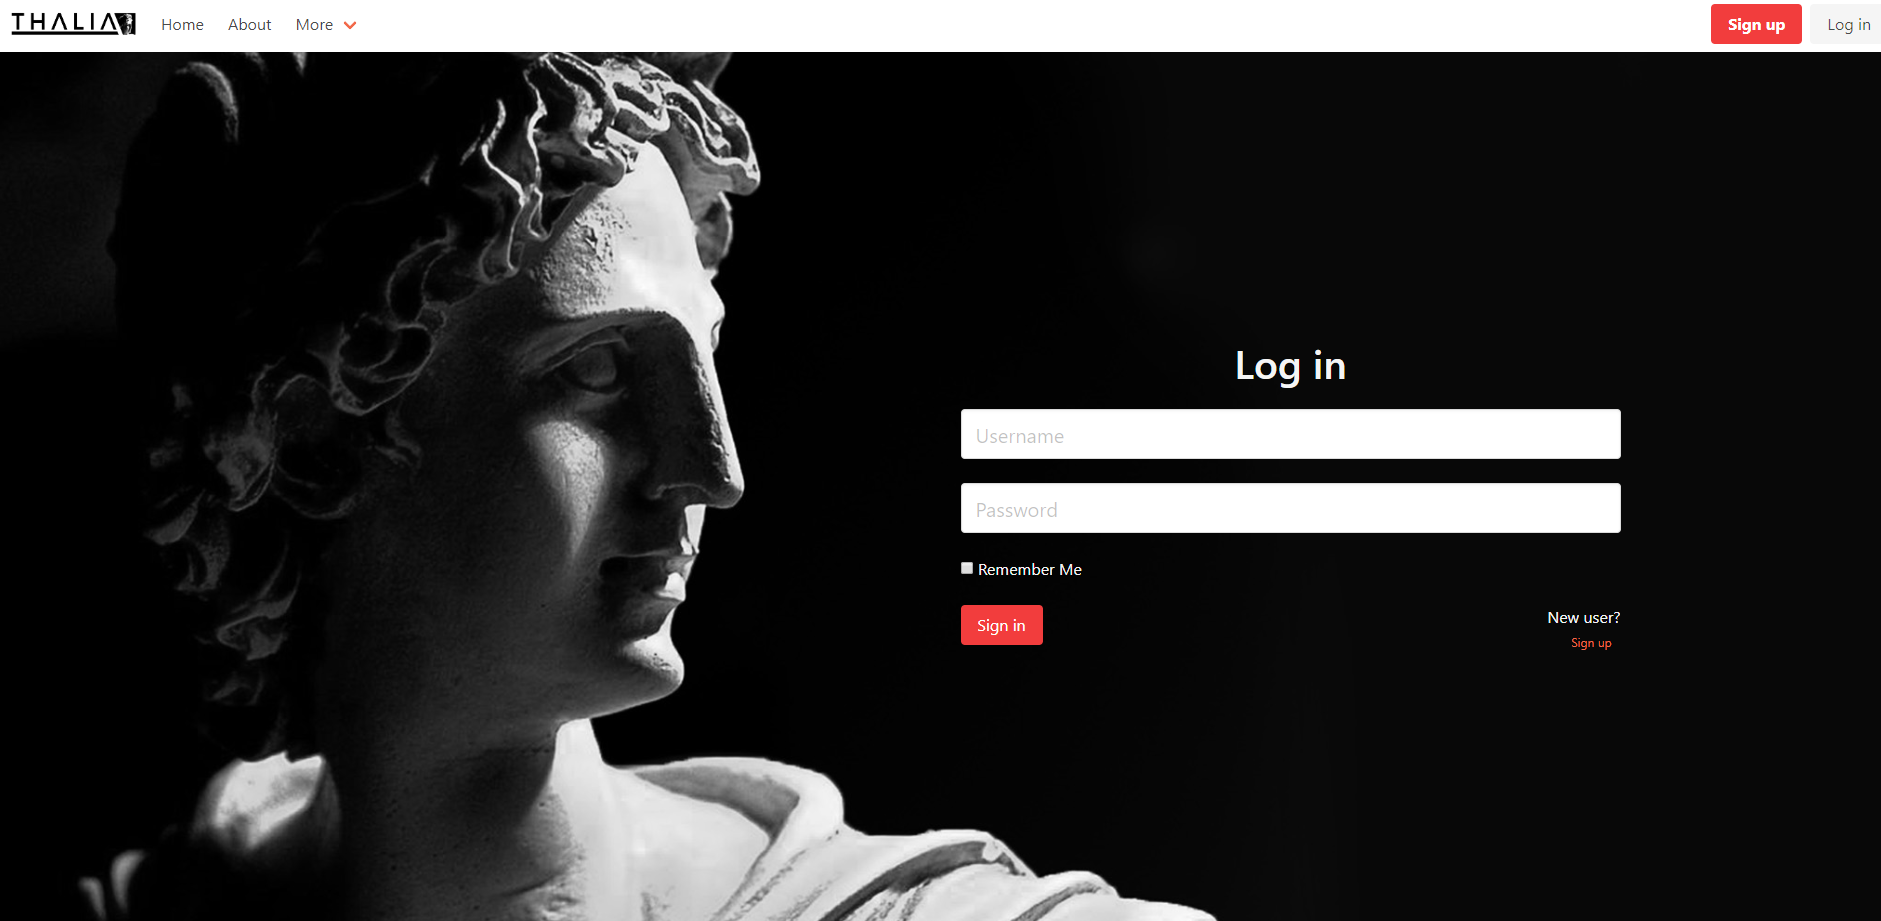
\includegraphics[width=\textwidth]{08Appendices/081User/081Pictures/login.png}
   \caption{Thalia Log In Page (source: TODO)}
   \label{thalia_login}
\end{figure}

In case the user is already logged in and attempts to access these pages, he or she gets redirected to the homepage. In addition the navbar changes to:

\begin{figure}[H]
   \centering
   \includegraphics[width=\textwidth]{08Appendices/081User/081Pictures/navbar_logged_in.png}
   \caption{Thalia Logout (source: TODO)}
   \label{thalia_navbar_logged_in}
\end{figure}

Opting to log out the user finds themselves at the homepage.

\subsubsection{Report Issues Page}

The Report Issues Page is available at \url{TODO} or via opening the dropdown menu on the navbar and clicking the link. This short form is for users to provide feedback, 
report possible issues or request features.

\begin{figure}[H]
   \centering
   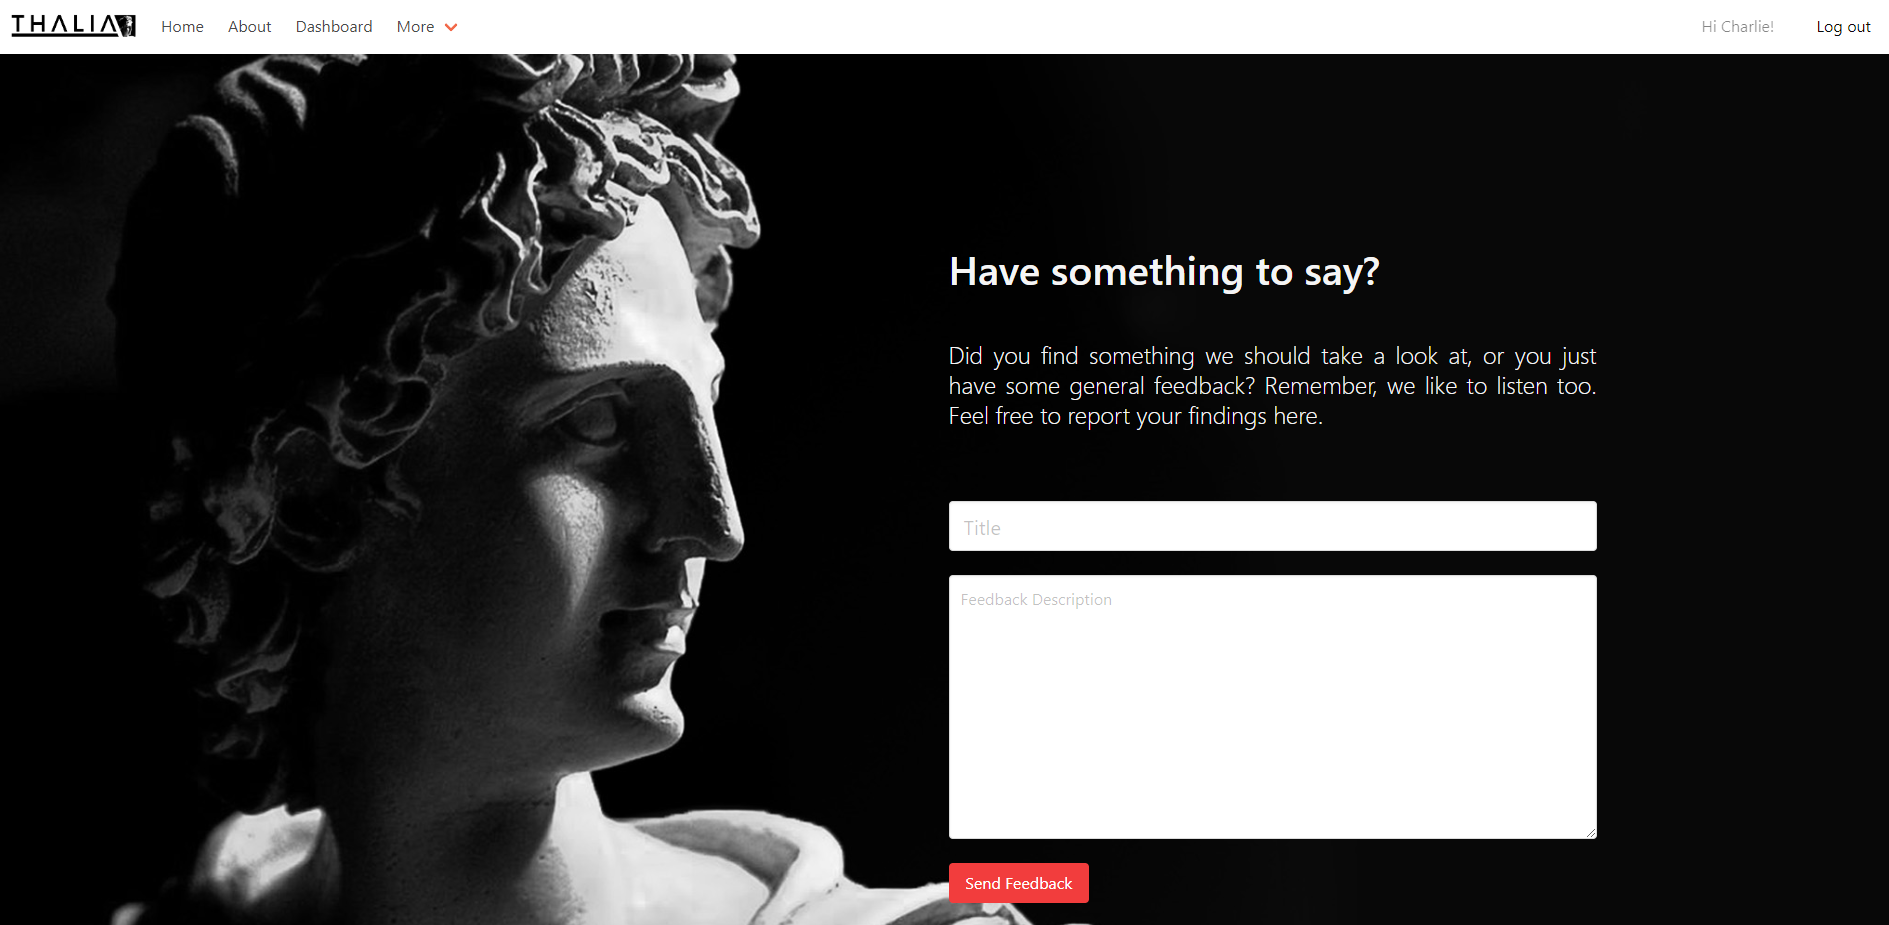
\includegraphics[width=\textwidth]{08Appendices/081User/081Pictures/issues.png}
   \caption{Thalia Report Issues Page (source: TODO)}
   \label{thalia_issues}
\end{figure}

\subsubsection{TODO PAGE}

\subsubsection{Dashboard}

The Dashboard, available only for logged in users is available at \url{TODO} or via the link on the navbar, is our main application. 
The webpage is divided into tabs, these are:

TODO
\begin{itemize}
    \item Ticker Selector
    \item Summary
    \item Metrics
    \item ...
\end{itemize}

At first only the Ticker Selector Page is accessible for the user. 
This is because the following tabs show only the output of backtesting a or multiple portfolios, and as a consequence are, for the time being, empty.

\begin{figure}[H]
   \centering
   
\includegraphics[width=\textwidth]{08Appendices/081User/081Pictures/disabled_tabs.png}
   \caption{Thalia Dashboard - Disabled Tabs (source: TODO)}
   \label{thalia_disabled_tabs}
\end{figure}

Let us now consider each tab individually. 

\subsubsubsection*{Ticker Selector}

Here the user is required to input their backtesting strategy. As Thalia supports testing multiple portfolios at once (up to 5 currently) there are input fields that are 
portfolio specific and that are not. The latter consists only of:

\begin{itemize}
    \item Start Date: The day the investment is made.
    \item End Date: The last day of the investment, defaulted to the present date.
    \item Initial Amount: Initial investment into the portfolio, default currency is dollars.
\end{itemize}

Although these values could also be made portfolio specific, it is unlikely that a user would want to compare portfolios with one of these values differing.
The portfolio specific input values are:

\begin{itemize}
    \item Portfolio Name: Defaulted to Portfolio 1, Portfolio 2, etc. 
    \item Contribution Amount: The sum of ...
    \item Contribution Frequency: How regularly should these contributions happen.
    \item Rebalancing Frequency: As a result ...
    \item Ticker Data: Discussed below.
\end{itemize}




\end{document}